%%%%%%%%%%%%%%%%%%%%%%%%%%%%%%%%
\section{Experiments}
\label{experiments}

%\begin{landscape}
\begin{figure*}[t]
% ensure that we have normalsize text
\normalsize
\begin{center}
\subfigure[Results of ICA methods in the case of mixture of images and Gaussian noise.] {\label{fig:rank1_a}
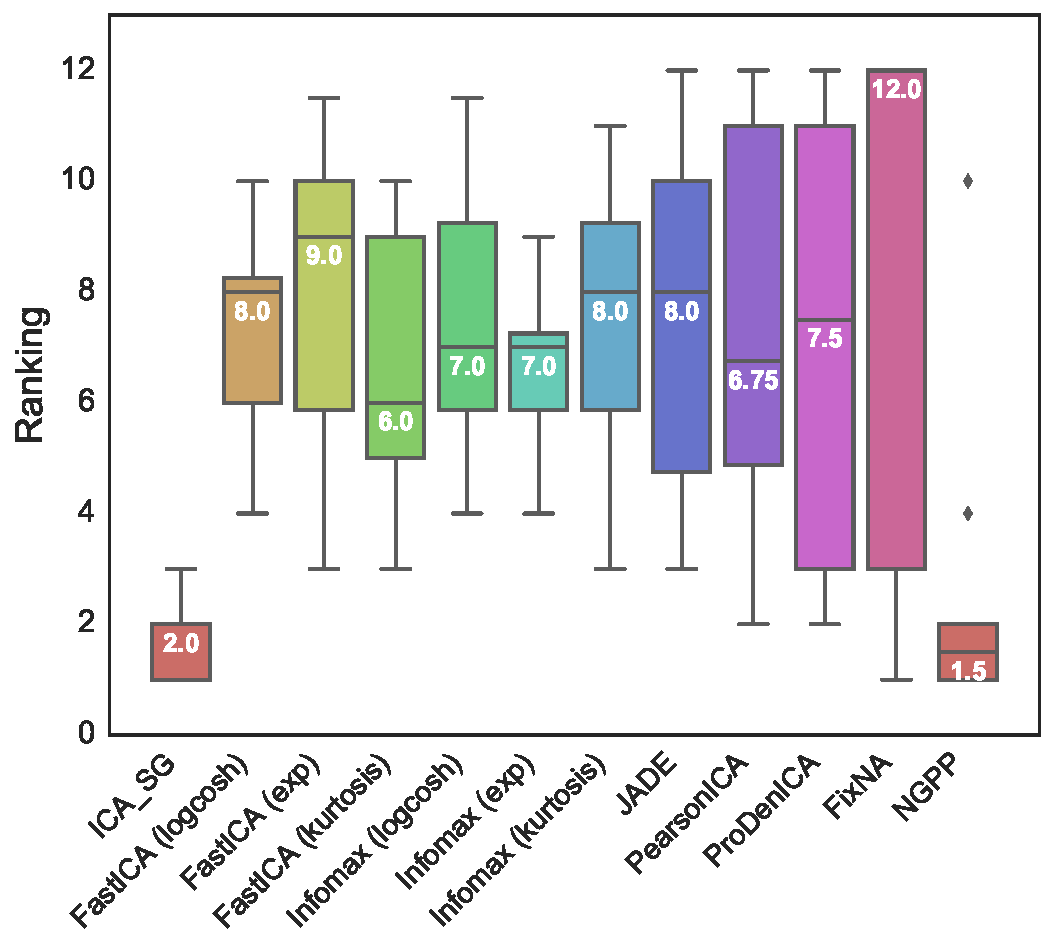
\includegraphics[width=2.2in]{ranking/images_boxplot-r1.pdf}
} \quad
\subfigure[Results of ICA methods in the case of mixture of images and salt and pepper \textbf{``salt and pepper''} noise.] {\label{fig:rank1_b}
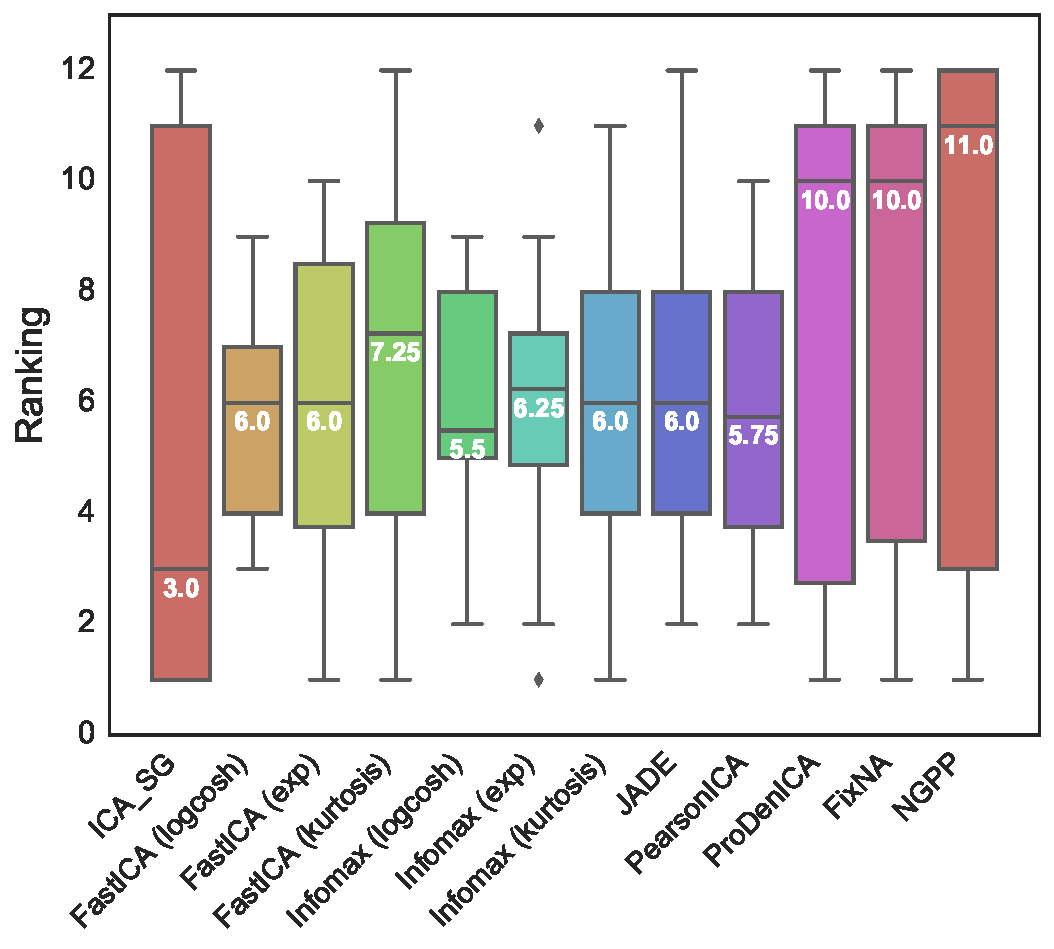
\includegraphics[width=2.2in]{ranking/images_boxplot-r2.pdf}
}\\
\end{center}
\caption{Results of ICA methods in the case of mixture of images and noise. \textbf{Moze nie powtarzac, jest juz w subcaptions to samo}}
\label{fig:rank1}
\end{figure*}

%\begin{landscape}
\begin{figure*}[t]
% ensure that we have normalsize text
\normalsize
\begin{center}
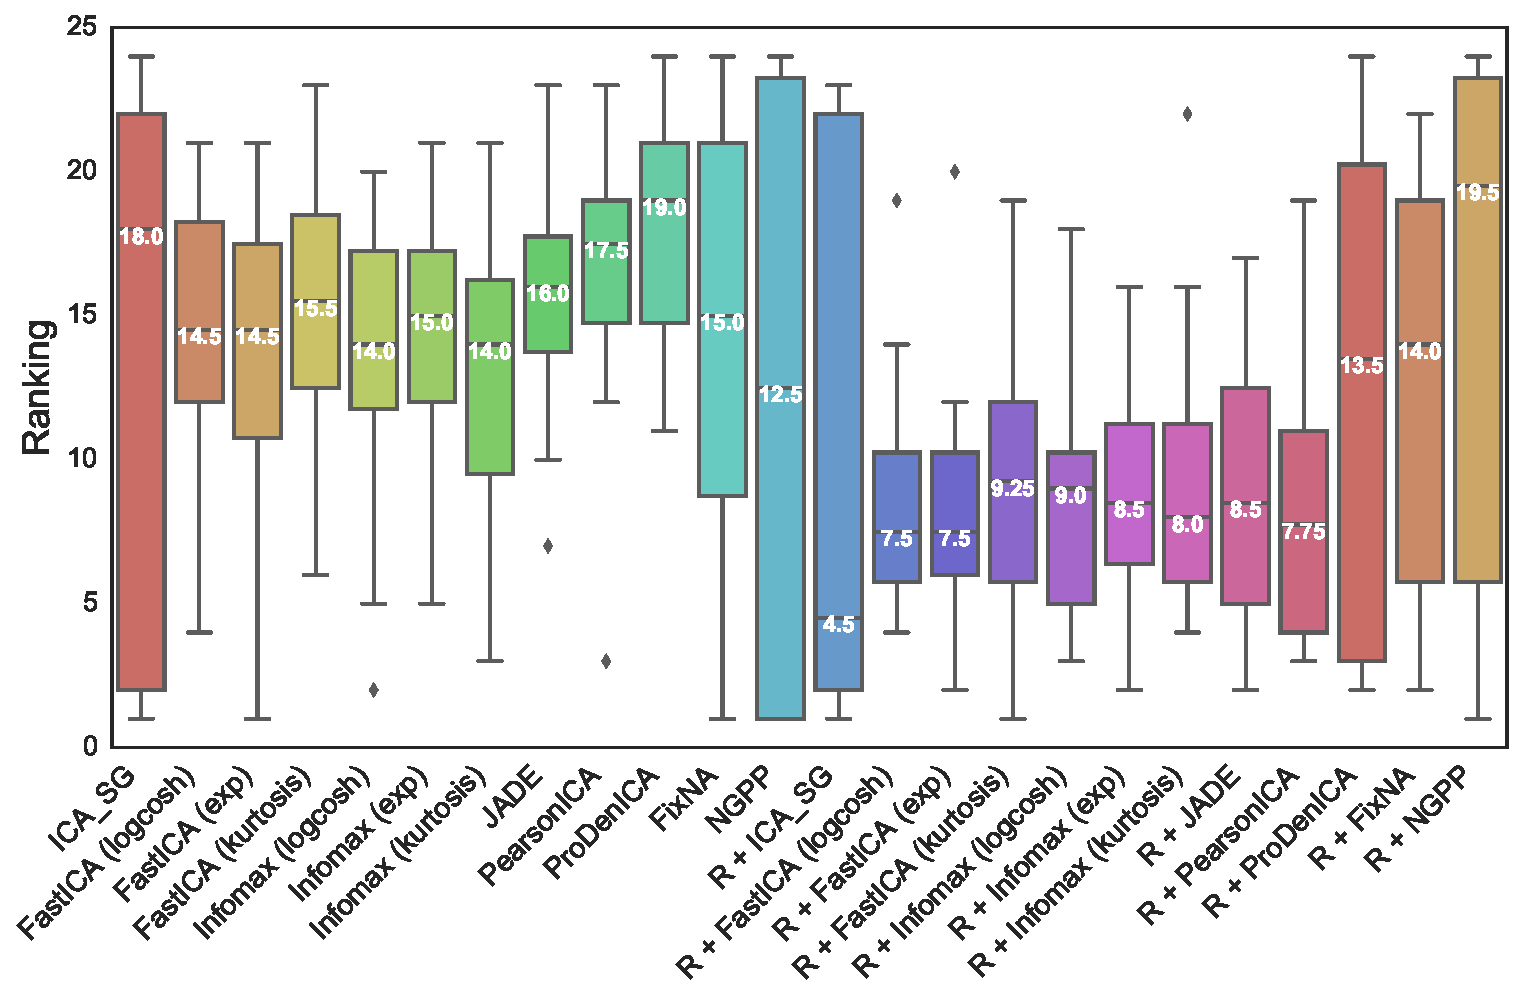
\includegraphics[width=4.0in]{ranking/images_boxplot-r3.pdf}
\end{center}
\caption{Results of ICA methods in the case of mixture of images and noise salt and pepper noise with scale (R+) and without preprocessing.}
\label{fig:rank2}
\end{figure*}

To compare \ICA{} to other state-of-the-art approaches we use 
Tucker's congruence coefficient \cite{lorenzo2006tucker} which values range between $-1$ and $+1$. It can be used to study the similarity of extracted factors across different samples. Generally, a congruence coefficient of $0.9$ indicates a high degree of factor similarity, while a coefficient of $0.95$ or higher indicates that the factors are virtually identical. 

We evaluate our method in the context of 2D and hyperspectral images. 
For comparison we use R package {\tt ica} \cite{ica}, {\tt PearsonICA} \cite{pearsonica}, {\tt ProDenICA} \cite{prodenica}, {\tt tsBSS} \cite{tsBSS}, {\tt NGPP} \cite{virta2016projection}.
The most popular method used in practice is FastICA \cite{hyvarinen1999fast,helwig2013critique} algorithm, which uses negentropy. In this context we can use three different functions to estimate neg-entropy:
logcosh, exp and kurtosis.
We also compare our method with algorithm using Information-Maximization (Infomax) approach \cite{bell1995information}. Similarly to FastICA we consider three possible non-linear functions: hyperbolic tangent, logistic and extended Infomax.
%We also consider algorithm which uses Joint Approximate Diagonalization of Eigenmatrices (JADE) proposed by Cardoso and Souloumiac's \cite{cardoso1993blind,helwig2013critique}.
%
%One of the most popular ICA methods dedicated for skew data is PearsonICA \cite{karvanen2000pearson,karvanen2002blind}, which minimizes mutual information using a Pearson \cite{stuart1968advanced} system-based parametric model. Another model we consider is ProDenICA \cite{bach2002kernel,hastie2009elements}, which is based not on a
%single nonlinear function, but on an entire function space of candidate nonlinearities. In particular, the method works with the functions in a reproducing kernel Hilbert space, and make use of the “kernel trick” to search over this space efficiently. 
%We also compare our method with  FixNA \cite{shi2009blind}, method for blind source separation problem.
%

%\begin{landscape}
\begin{figure*}[t]
% ensure that we have normalsize text
\normalsize
\begin{center}
  \subfigure[Original images 42049 and 220075 and Gaussian nice \textbf{noise}.] {\label{fig:image_ICA_res_1}
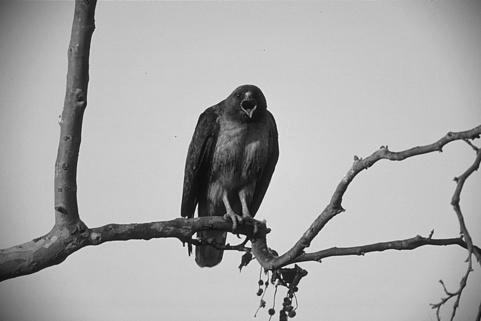
\includegraphics[width=1.4in]{3/2_6_or_1} 
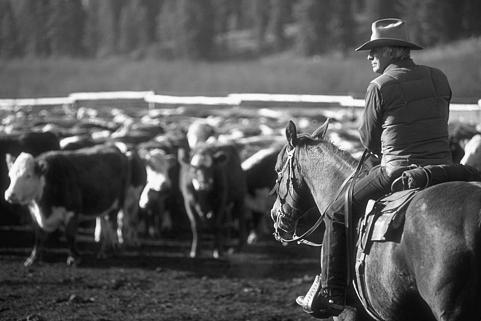
\includegraphics[width=1.4in]{3/2_6_or_2}
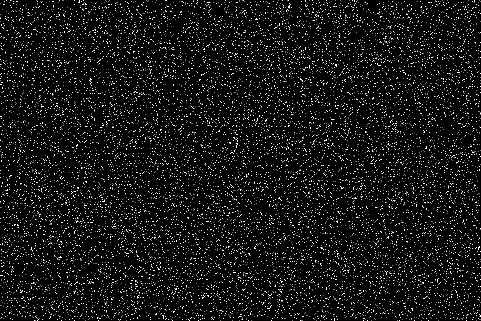
\includegraphics[width=1.4in]{3/2_6_or_3}
}
%\subfigure[Mixture of sources.] {\label{fig:image_ICA_res_1}
%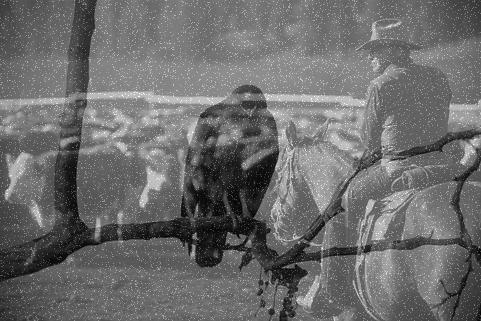
\includegraphics[width=0.9in]{3/2_6_div_1} 
%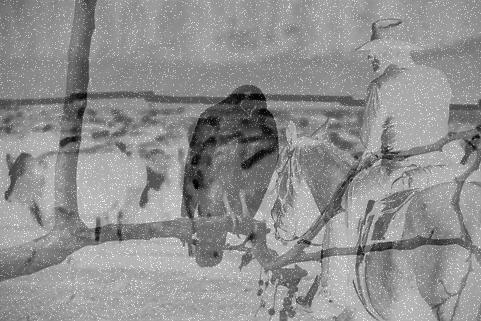
\includegraphics[width=0.9in]{3/2_6_div_2}
%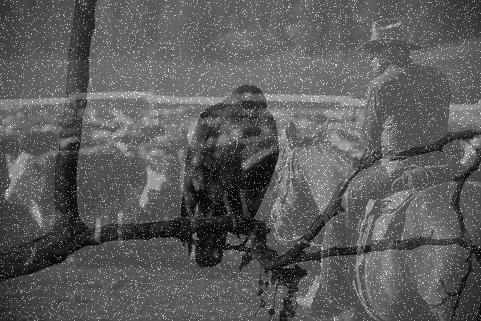
\includegraphics[width=0.9in]{3/2_6_div_3}
%}
\subfigure[Mixture of sources after rescaling.] {\label{fig:image_ICA_res_1}
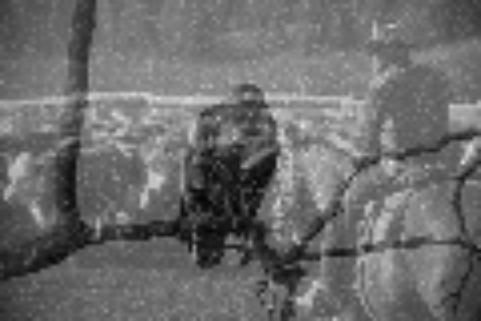
\includegraphics[width=1.4in]{3/2_6_div_1_r} 
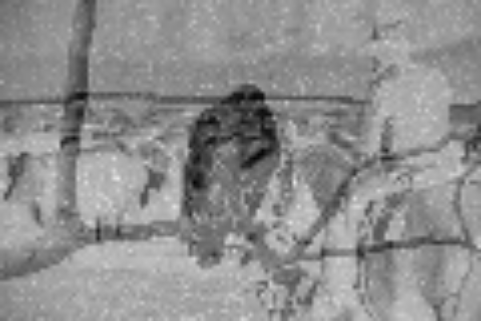
\includegraphics[width=1.4in]{3/2_6_div_2_r}
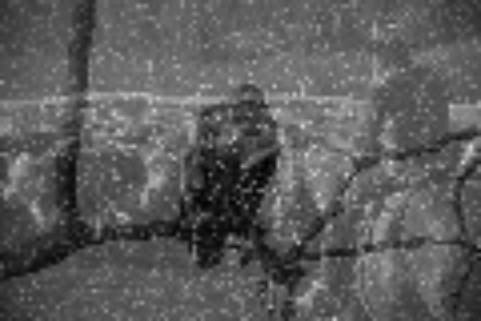
\includegraphics[width=1.4in]{3/2_6_div_3_r}
}

%%%%%%%%%%%%%%%%%%%%
%\subfigure[Sum and subtraction of images.] {\label{fig:image_ICA_int_2}
%\includegraphics[width=1.2in]{2/2_6_sum} 
%\includegraphics[width=1.2in]{2/2_6_div}
%} \\

%%%%%%%%%%%%%%%%%%%%
\subfigure[\ICA.] {\label{fig:image_ICA_res_3}
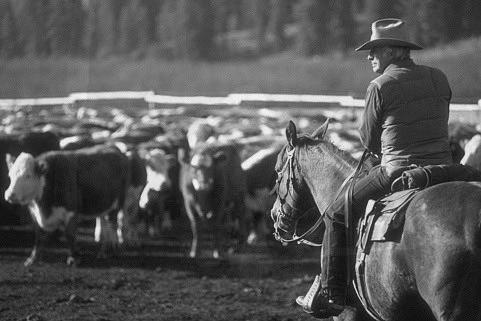
\includegraphics[width=1.in]{3/2_6_SGD_2} 
}
\subfigure[FastICA.] {\label{fig:image_ICA_res_4}
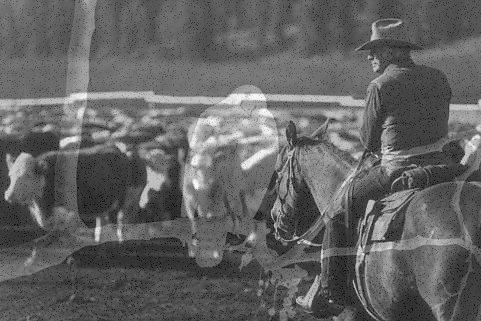
\includegraphics[width=1.in]{3/2_6_ICA11_2} 
}
\subfigure[ProDenICA.] {\label{fig:image_ICA_res_5}
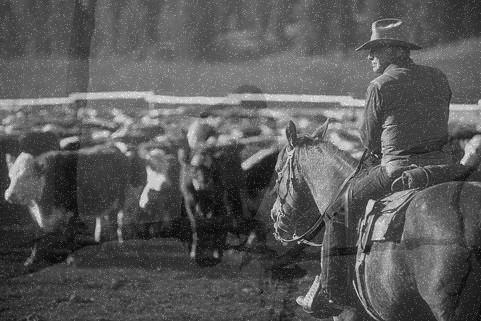
\includegraphics[width=1.in]{3/2_6_ICA5_2} 
}
\subfigure[NGPP.] {\label{fig:image_ICA_res_9}

\includegraphics[width=1.in]{3/2_6_ICA8_1}
}\\
%%%%%%%%%%%%%%%%%%%%

\subfigure[\ICA.] {\label{fig:image_ICA_res_6}
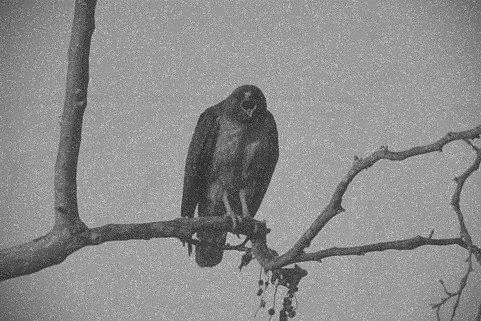
\includegraphics[width=1.in]{3/2_6_SGD_1}
}
\subfigure[FastICA.] {\label{fig:image_ICA_res_7}
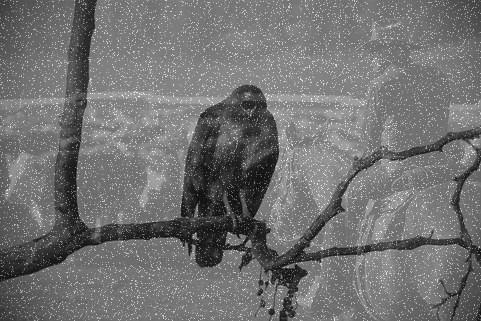
\includegraphics[width=1.in]{3/2_6_ICA11_1}
}
\subfigure[ProDenICA.] {\label{fig:image_ICA_res_8}
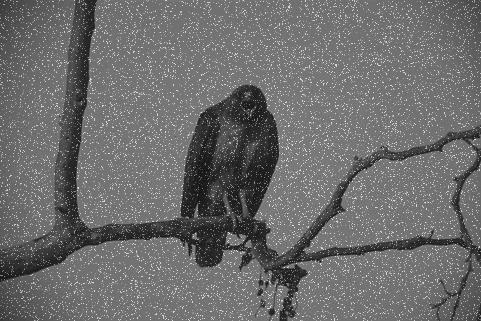
\includegraphics[width=1.in]{3/2_6_ICA5_1}
}
\subfigure[NGPP.] {\label{fig:image_ICA_res_10}
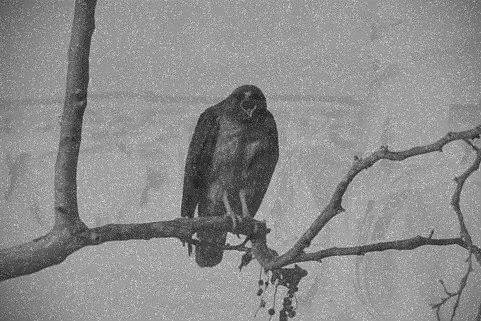
\includegraphics[width=1.in]{3/2_6_ICA8_2}
}
\end{center}
\caption{Comparison of images separation by our method (\ICA), with FastICA,  ProDenICA, NGPP. \textbf{Ale to jest to samo co Fig.1 -- po co powtarzac?} }
\label{fig:image_ICA_res}
\end{figure*}


\subsection{Separation of images}

One of the most popular application of ICA is the separation of images. In our experiments we use four images from the USC-SIPI Image Database of size $256 \times 256$ pixels (4.1.01, 4.1.06, 4.1.02, 4.1.03) and eight of size $512 \times 512$ pixels (4.2.04, 4.2.02, boat.512, elaine.512, 5.2.10, 5.2.08, 5.3.01, 4.2.03). We also use 8 images from the Berkeley Segmentation Dataset of size $482 \times 321$ with indexes (\#119082, \#42049, \#43074, \#38092, \#157055, \#220075, \#295087, \#167062). 

We make random pairs of above images and one component with noise (random sample from Gaussian distribution $\nor(0,1)$) and use them as a source signal combined by the mixing matrix $A = \begin{bmatrix} 1 & 1 & 1  \\ 1 & -1 & -1 \\ -1 & 1 & -1  \end{bmatrix} $. Our goal was to reconstruct two original images by using only the knowledge about mixed ones. The visualization of this process we present in Fig. \ref{fig:image_ICA_int}. 

\begin{table*}[t]
\label{tab:congru_img_1}
\vskip 0.15in
\begin{center}
\begin{small}
\begin{sc}
\resizebox{\textwidth}{!}{
\begin{tabular}{ c | c c c c c c c c  c  c  c  c c}
\hline
%\abovespace\belowspace
 & \ICA  & FastICA & FastICA & FastICA & Infomax & Infomax & Infomax & JADE & PearsonICA & ProDenICA & \ \  FixNA & \ \ NGPP\\ 
  &  &  logcosh & exp & kurtosis & tanh & tangent & logistic &  & & & & \\
\hline
%\abovespace
Source 1 & 0.3427 & 0.2778 & 0.2820 & 0.2865 & 0.2823 & 0.2731 & 0.2979 & 0.2901 & 0.2837 & 0.2065 & 0.1827 & 0.1820 \\
Source 2 & 0.3212 & 0.4122 & 0.3954 & 0.3690 & 0.4168 & 0.4193 & 0.1972 & 0.3611 & 0.2679 & 0.1318 & 0.3020 & 0.3176 \\
Source 3 & 0.3180 & 0.1857 & 0.1878 & 0.1285 & 0.1845 & 0.1819 & 0.3782 & 0.0053 & 0.0252 & 0.2565 & 0.0426 & 0.2962 \\
Source 4 & 0.2822 & 0.0357 & 0.0364 & 0.1743 & 0.0339 & 0.0208 & 0.0317 & 0.1780 & 0.2802 & 0.1724 & 0.3196 & 0.1768 \\

\hline
\end{tabular}
}
\end{sc}
\end{small}
\end{center}
\caption{Tucker's congruence coefficients between average edges form reference layers and various ICA results.}
\end{table*}

As a summary from the experiment, in Figure \ref{fig:rank1_a} we present a boxplot \textbf{czy miales na mysli box plots?} of \textbf{the} ranks obtained by the methods.
The \ICA {} almost perfectly recovered source signal and it is one of the best in ranking. 
Although this is not surprising as the experiments were in fact conducted in the setting which favored our approach, as we chose the noise to be gaussian, \textbf{Znowu sie kajamy, czy potrzebnie to spytaj Jacka. Ale jakos niezgrabnie?} this shows that \ICA{} works as desired and deals well with removing \textbf{any} gaussian components from the data. 

In the next experiments we reaped \textbf{repeated?} the procedure with salt and pepper \textbf{``salt and pepper''} noise. But \textbf{usun But} before applying ICA methods we rescale images, see Fig. \ref{fig:image_ICA_res}. 
Such procedure can be understand as a preprocessing in the ICA framework. After rescaling of images non-gaussian noise become more normal and therefore we are able to remove them. In Figure \ref{fig:rank1_a} we present a boxplot \textbf{box plot? box plots? box-plot?} of ranks obtained on rescale data \textbf{on the rescaled data}. 

The rescaling of images give sensational \textbf{lepiej vastly zamiast sensational} better results in the case of non-gaussian noise end increase \textbf{and increases the} score of all methods, see Figure \ref{fig:rank2}. 


%\begin{landscape}
\begin{figure*}[t!]
% ensure that we have normalsize text
\normalsize
\begin{center}
%\subfigure[The effect of the \ICA \ method.] {\label{fig:image_1}
%  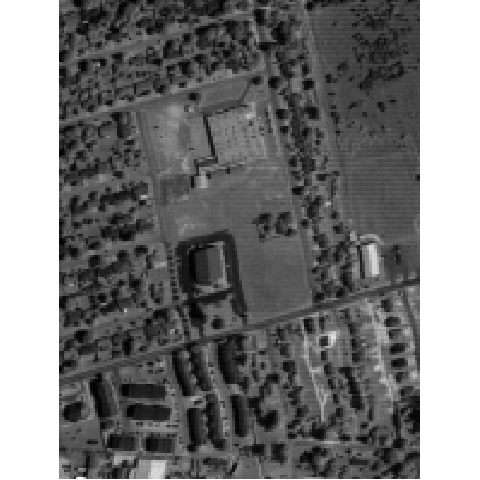
\includegraphics[width=1.2in]{spec/1a} 
%  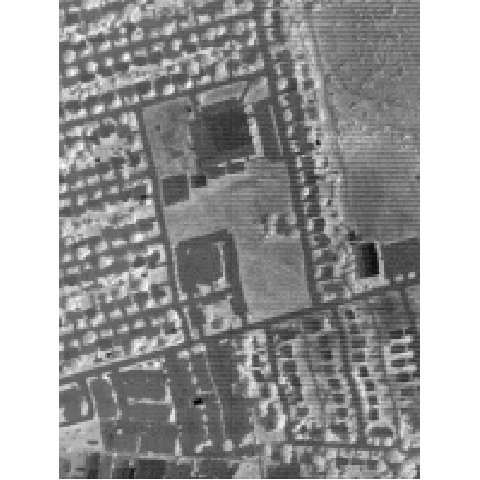
\includegraphics[width=1.2in]{spec/2a}
%  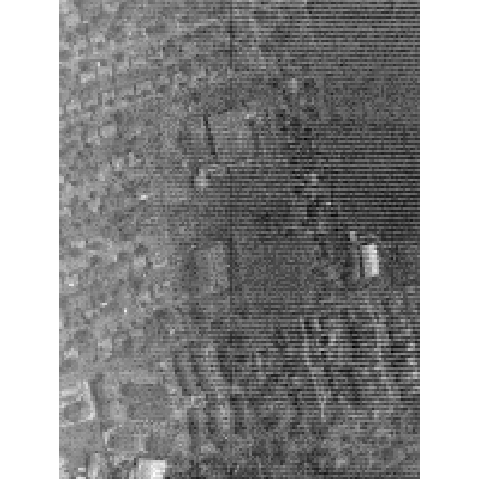
\includegraphics[width=1.2in]{spec/3a} 
%  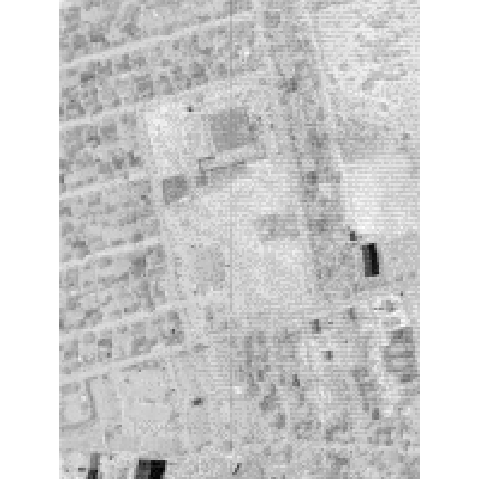
\includegraphics[width=1.2in]{spec/4a}
%} \\
%%%%%%%%%%%%%%%%%%%%%%%%%%%%%%%%%%
%%%%%%%%%%%%%%%%%%%%%%%%%%%%%%%%%%
\subfigure[Ground truth layers which contains 4 channels: \#1 Asphalt, \#2 Grass, \#3 Tree and \#4 Roof.] {\label{fig:image_1}
  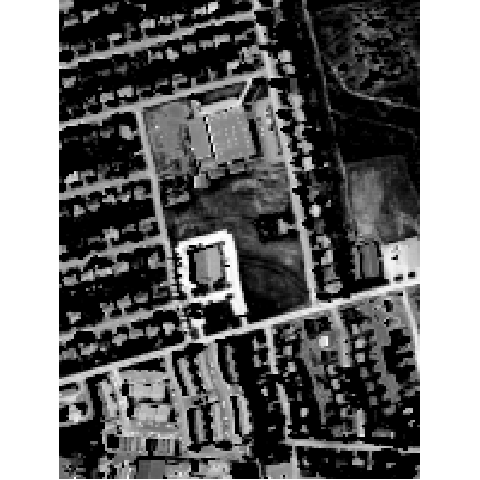
\includegraphics[width=1.in]{spec/O_1} 
  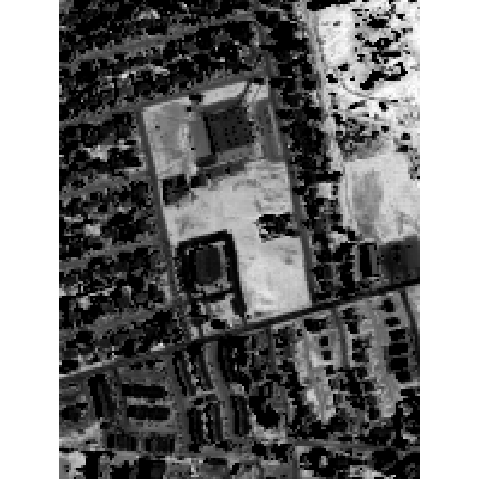
\includegraphics[width=1.in]{spec/O_2}
  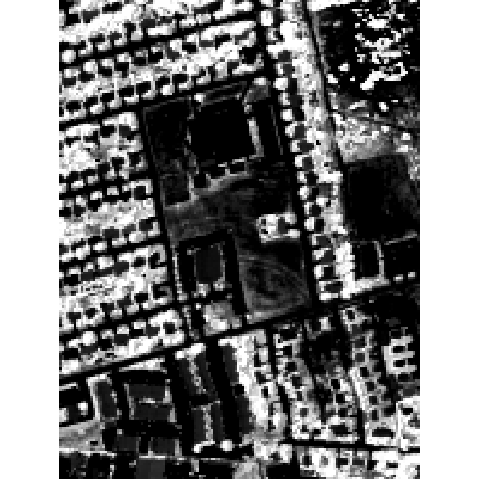
\includegraphics[width=1.in]{spec/O_3} 
  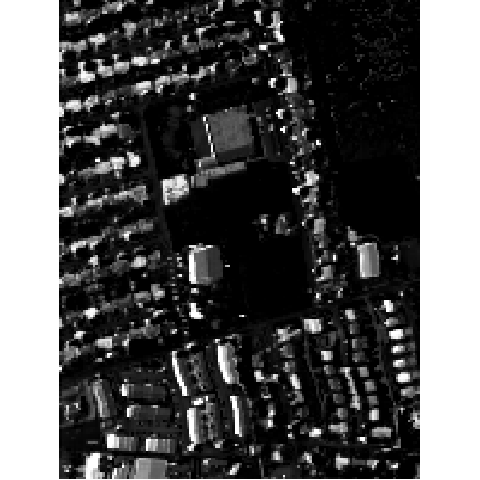
\includegraphics[width=1.in]{spec/O_4}
} \\
%%%%%%%%%%%%%%%%%%%%%%%%%%%%%%%%%%
%%%%%%%%%%%%%%%%%%%%%%%%%%%%%%%%%%
\subfigure[The effect of the \ICA \ method.] {\label{fig:image_2}
  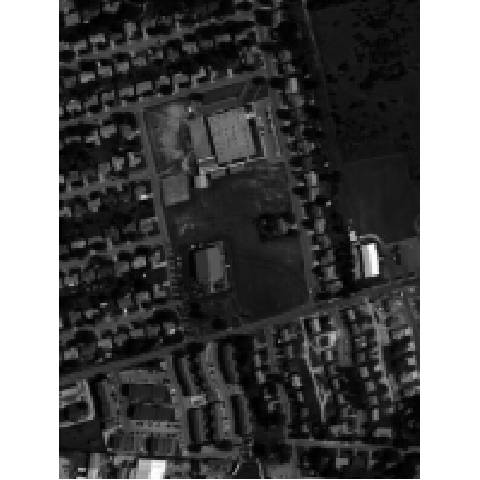
\includegraphics[width=1.in]{spec/SG_1} 
  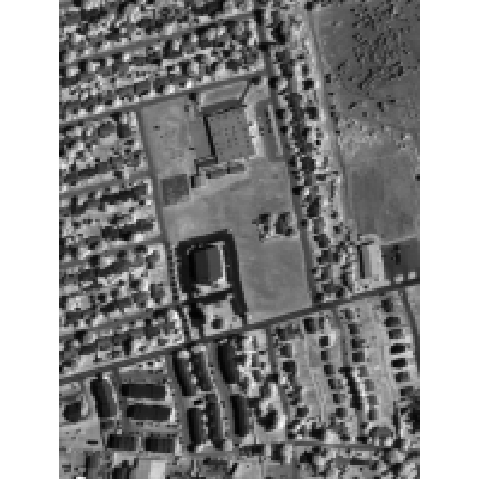
\includegraphics[width=1.in]{spec/SG_2}
  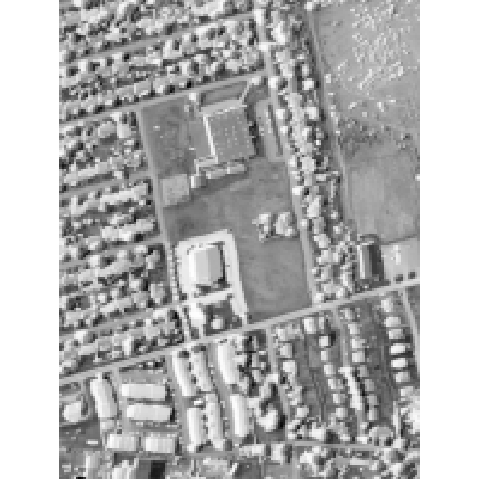
\includegraphics[width=1.in]{spec/SG_3} 
  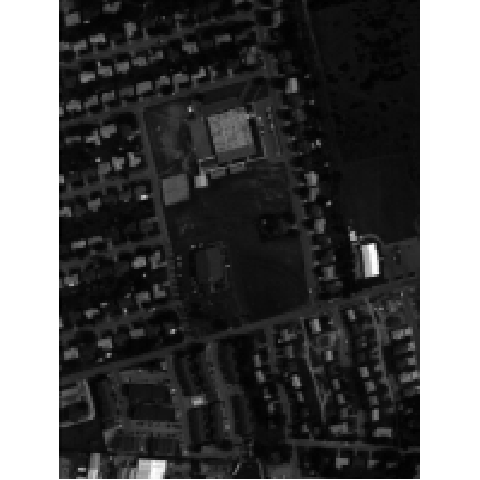
\includegraphics[width=1.in]{spec/SG_4}
} \\
%%%%%%%%%%%%%%%%%%%%%%%%%%%%%%%%%%
%%%%%%%%%%%%%%%%%%%%%%%%%%%%%%%%%%
\subfigure[The effect of the FastICA (logcosh) method.] {\label{fig:image_3}
  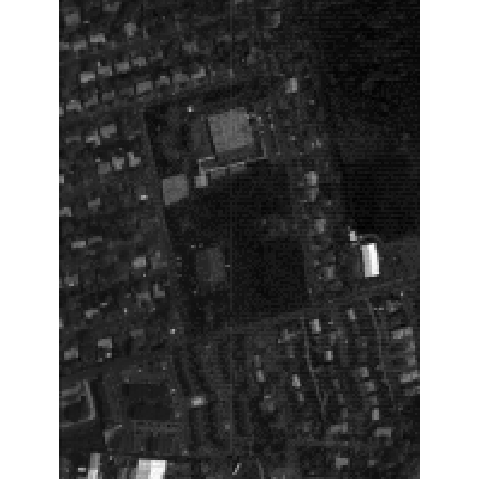
\includegraphics[width=1.in]{spec/ICA11_3} 
  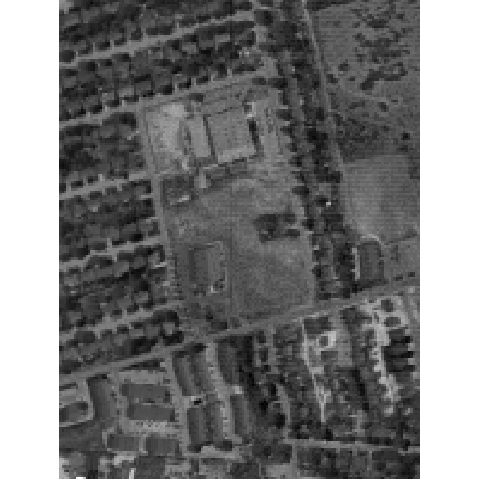
\includegraphics[width=1.in]{spec/ICA11_2}
  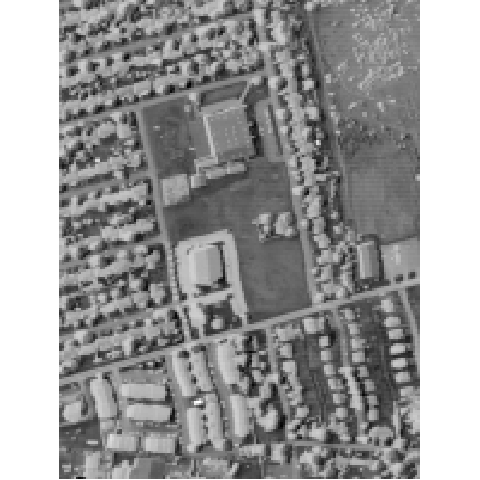
\includegraphics[width=1.in]{spec/ICA11_1} 
  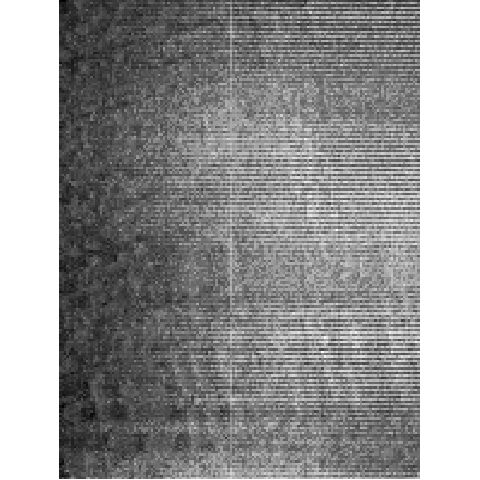
\includegraphics[width=1.in]{spec/ICA11_4}
} \\
%%%%%%%%%%%%%%%%%%%%%%%%%%%%%%%%%%
%%%%%%%%%%%%%%%%%%%%%%%%%%%%%%%%%%
%\subfigure[The effect of the PearsonICA method.] {\label{fig:image_1}
%  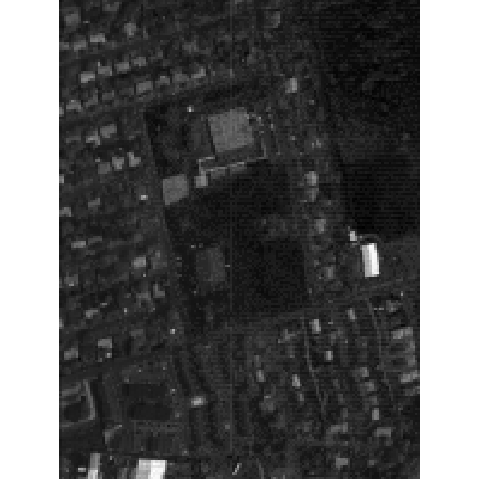
\includegraphics[width=1.2in]{spec/ica_41} 
%  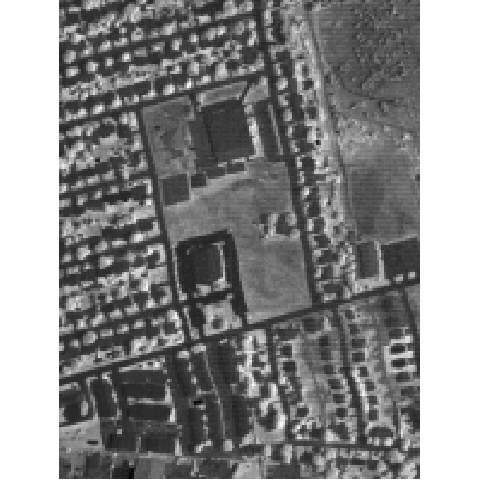
\includegraphics[width=1.2in]{spec/ica_42}
%  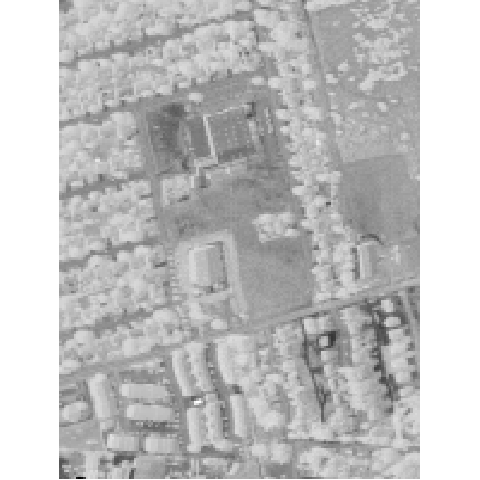
\includegraphics[width=1.2in]{spec/ica_43} 
%  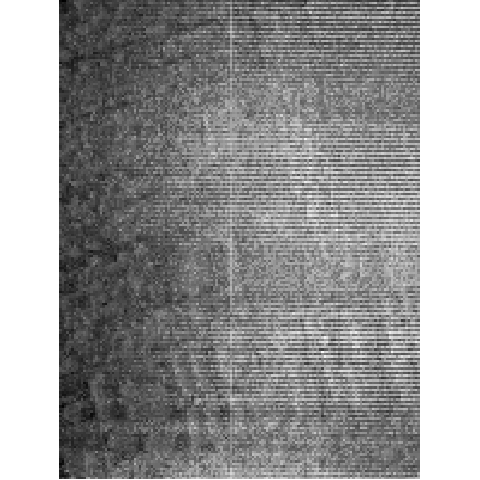
\includegraphics[width=1.2in]{spec/ica_44}
%} \\
%%%%%%%%%%%%%%%%%%%%%%%%%%%%%%%%%%
%%%%%%%%%%%%%%%%%%%%%%%%%%%%%%%%%%
\subfigure[The effect of the  ProDenICA method.] {\label{fig:image_4}
  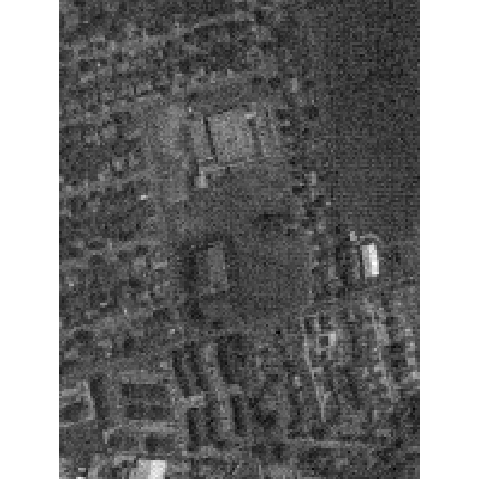
\includegraphics[width=1.in]{spec/ICA5_1} 
  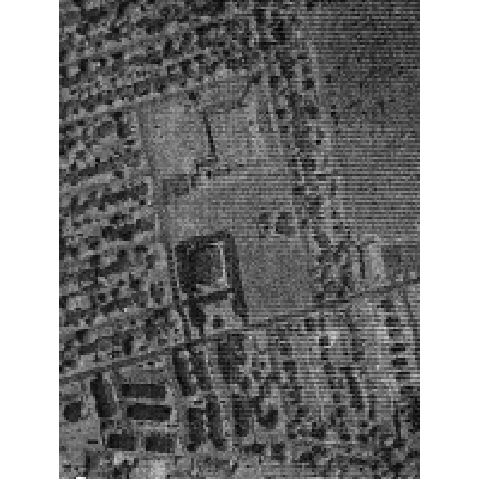
\includegraphics[width=1.in]{spec/ICA5_4}
  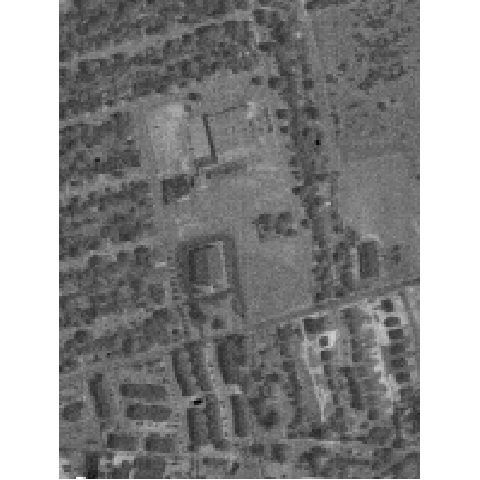
\includegraphics[width=1.in]{spec/ICA5_3} 
  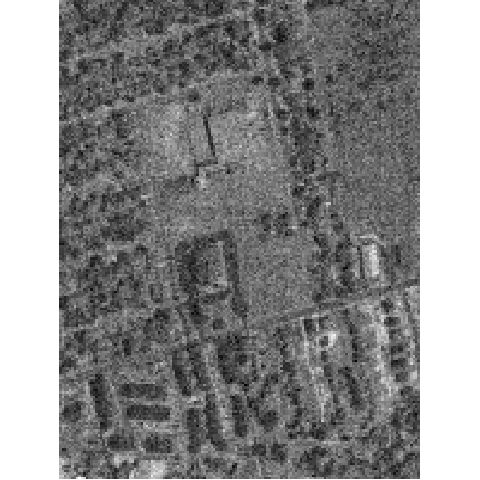
\includegraphics[width=1.in]{spec/ICA5_2}
} \\
%%%%%%%%%%%%%%%%%%%%%%%%%%%%%%%%%%
%%%%%%%%%%%%%%%%%%%%%%%%%%%%%%%%%%
\subfigure[The effect of the  NGPP method.] {\label{fig:image_5}
  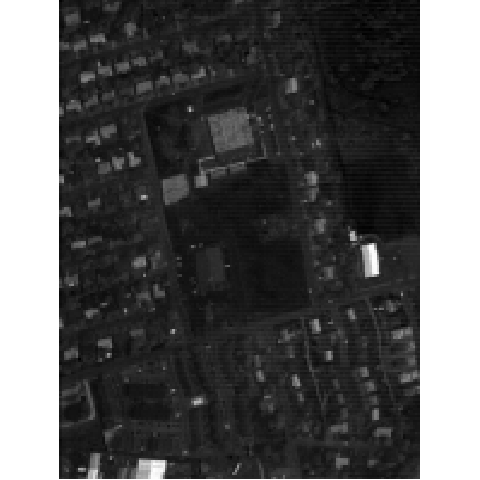
\includegraphics[width=1.in]{spec/ICA8_1} 
  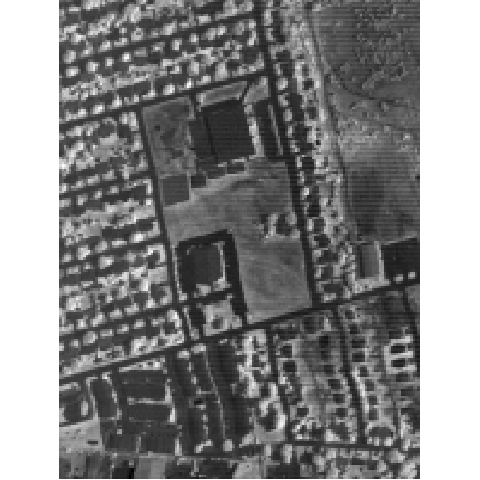
\includegraphics[width=1.in]{spec/ICA8_2}
  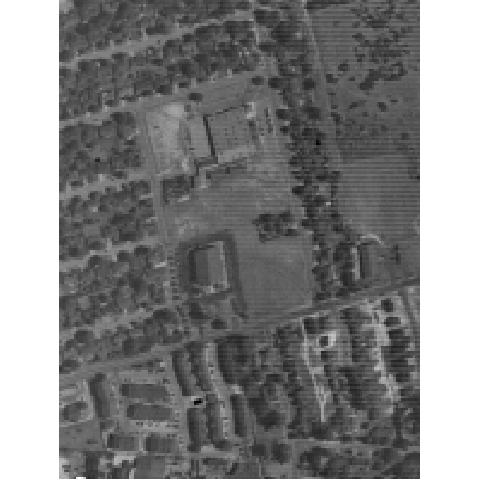
\includegraphics[width=1.in]{spec/ICA8_3} 
  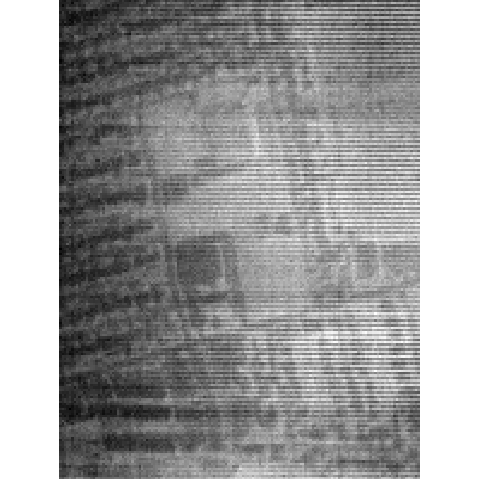
\includegraphics[width=1.in]{spec/ICA8_4}
} 
\end{center}
\caption{Results of image separation with the uses of various ICA algorithms.}
\label{fig:spec_1}
\end{figure*}


\subsection{Hyperspectral Unmixing}

Independent component analysis has been recently \textbf{can be zamiast has been recently?}
applied into \textbf{to zamiast into} hyperspectral unmixing 
\cite{wang2015abundance}
as a result of \textbf{lepiej due to} its low
computation time and its ability to perform without prior information.
In this subsection we apply \textbf{present a zamiast apply} simple example which suggests that our method also can by used for spectral data.

Urban data  \cite{fyzhu2014IJPRSSSNMF,fyzhu2014TIPDgSNMF,fyzhu2014JSTSPRRLbSF} is one of the most widely used hyperspectral data-sets used \textbf{usun used} in the hyperspectral \textbf{usun hyperspectral} unmixing study. Each image has $307 \times 307$ pixels, each of which corresponds to a $2 \times 2$ m area. In this image, there are 210 wavelengths ranging from 400 nm  to 2500 nm, resulting in a spectral resolution of 10 nm. After the channels 1--4, 76, 87, 101--111, 136--153 and 198--210 are removed (due to dense water vapor and atmospheric effects), there remain 162  channels (this is a common preprocess for hyperspectral unmixing analyses). There is ground truth \cite{fyzhu2014IJPRSSSNMF,fyzhu2014TIPDgSNMF,fyzhu2014JSTSPRRLbSF}, which contains 4 channels: \#1 Asphalt, \#2 Grass, \#3 Tree and \#4 Roof.

A highly mixed area is cut from the original data set in this experiment (similar example was showed in \cite{wang2015abundance}), with the size of $200 \times 150$ pixels. %Fig. \ref{} shows the true-color image. 

In our experiment we compared \ICA{} to other popular ICA methods, see Fig. \ref{fig:spec_1}. Observe that \ICA{}, NGPP and ProDenICA give layers which seem to contain more information then FastICA, as the last component in FastICA contains mainly noise. To verify which method separate sources from noise better we calculate how obtained layers corresponds to original signals. Since there is no classical measure for such task \textbf{przecinek} we verified it by calculation \textbf{calculating the} correlation coefficient between \textbf{the} average muse \textbf{co to jest muse? moze literowka a moze ja nie znam slowa} of edges of reference layers (in our experiment we use Canny edge detector \textbf{zrob z tego osobne zdanie}) and ICA results, see Tab. \ref{tab:congru_img_1}. Our method gives similar \textbf{comparable zamiast similar} value of similarity measure on all layers. 


%
%\begin{table*}[t]
%\caption{Classification accuracies for naive Bayes and flexible 
%Bayes on various data sets.}
%\label{tab:congru_img_1}
%\vskip 0.15in
%\begin{center}
%\begin{small}
%\begin{sc}
%\resizebox{\textwidth}{!}{
%\begin{tabular}{ c c c c c c c c c  c  c  c  c }
%\hline
%%\abovespace\belowspace
% & \ICA  & FastICA & FastICA & FastICA & Infomax & Infomax & Infomax & JADE & PearsonICA & ProDenICA \\ 
%  &  &  logcosh & exp & kurtosis & tanh & tangent & logistic &  & &  \\
%\hline
%%\abovespace
%
%\hline
%\end{tabular}
%}
%\end{sc}
%\end{small}
%\end{center}
%\vskip -0.1in
%\end{table*}

%\begin{table*}[!t]
%\centering
%\scalebox{0.7}{ 
%\begin{tabular}{ | c | c  | c c c | c c c | c | c | }
%\multicolumn{1}{c}{} & \multicolumn{1}{c}{\ICA}  & \multicolumn{3}{c}{FastICA} & \multicolumn{3}{c}{Infomax}  & \multicolumn{1}{c}{PearsonICA} & \multicolumn{1}{c}{ProDenICA}  \\ 
% &  &  logcosh & exp & kurtosis & tanh & tangent & logistic & &  \\
%\hline
%\#1 Asphalt  &\bf 0.6774 &  0.2859 & 0.2864 & -0.2595 & -0.2972 & -0.2954 &  -0.2972 &  0.20978 & 0.4928  \\
%\#2 Grass  & \bf -0.7784 &  -0.2746 & -0.2605 &  -0.2798 &  -0.2814 & -0.2816 & -0.2814 &  -0.2412 & -0.4323  \\
%\#3 Tree  & \bf 0.7267 & 0.2338 &  0.2717 &  -0.2547 &  0.2441 & 0.2354 &  0.2442 &   0.2482 & -0.5961  \\
%\#4 Roof &\bf 0.6666 &  -0.4256 &  0.4279 &  0.4167 & -0.4244 &  0.4301 & -0.4244 &  0.4193 &  -0.6128  \\
%
%\end{tabular}
%}
%\caption{The Tucker's congruence coefficient measure between reference layers and results of different ICA algorithms in the case of the urban data set.}
%\label{tab:spec}
%\end{table*}


%\begin{figure*}[!t]
%\normalsize
%\begin{center}
%\includegraphics[width=5in]{spec_1}
%\end{center}
%\caption{Congruence distance between layers obtain by different ICA algorithms and the closest reference channel.}
%\label{fig:spec_1}
%\end{figure*}




